\section{Perancangan Sistem}
Sistem \emph{question answering} yang akan dibangun menggunakan platform Java dengan metode pemrograman berorientasi objek, untuk itu pemodelan sistem menggunakan bahasa UML \emph{(Unified Modelling Language)}. Adapun diagram UML yang digunakan untuk merepresentasikan sistem adalah \emph{usecase diagram, activity diagram, sequence diagram dan state diagram}. 

\subsection{Diagram \emph{usecase}}
Diagram \emph{usecase} digunakan untuk menunjukkan interaksi sistem dengan aktor atau pengguna, berapa jumlah aktor serta hak akses masing-masing aktor terhadap sistem. Gambar \ref{fig:usecase_diagram} menunjukkan hubungan antara aktor dengan sistem. Sistem \emph{question answering} yang akan dibangun hanya melibatkan satu aktor yaitu pengguna yang akan memasukkan pertanyaan.
\begin{figure}[h]
    \centering
    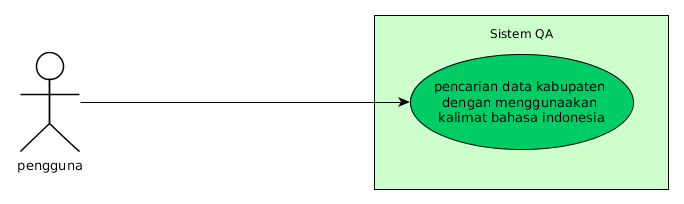
\includegraphics[width=0.8\textwidth]{usecase_diagram}
    \caption{Diagram \emph{usecase} sistem \emph{question answering}}
    \label{fig:usecase_diagram}
\end{figure}

\subsection{Diagram kelas}
Sistem \emph{question answering} yang akan dikembangkan memiliki beberapa kelas yang dibagi ke dalam beberapa paket utama yaitu paket controllers, models dan helpers.

\subsubsection{Kelas \emph{Main}}
Kelas \emph{Main} merupakan kelas yang berfungsi sebagai \emph{controller} yang bertugas untukmengatur komunikasi antara \emph{client} dengan server. Kelas ini merupakan sub kelas dari httpServlet. Kelas \emph{Main} diletakkan dalam paket \emph{controller} sedangkan kelas httpServlet berada pada paket \emph{javax.servlet.http}

Kelas Main terdiri dari dua buah method yaitu \emph{doGet()} dan \emph{processRequest()}. \emph{doGet()} memiliki akses kenampakan \emph{protected} dan merupakan versi \emph{overriding} dari method \emph{doGet()} pada kelas httpServlet. Method \emph{processRequest()} memiliki akses kenampakan private sehingga tidak dapat diakses dari luar atau dari web karena method ini hanya berfungsi sebagai pemroses internal yang hanya akan dipanggil melalui internal kelas Main.

\subsubsection{Kelas Tokenizer}
Tokenizer merupakan kelas yang berfungsi untuk melakukan proses tokenisasi terhadap kalimat tanya yang dikirimkan oleh user. Tokenizer akan menghasilkan data token berupa \emph{array list}
\subsubsection{Kelas NGram}
Kelas ini berfungsi untuk melakukan proses penggabungan kata per kata untuk kemudian di cek pada ontologi apakah kata yang terbentuk terdapat di dalam ontologi atau tidak. Kelas ini juga berfungsi untuk melakukan POS-Tangging terhadap token untuk menandakan tipe dari kata tersebut.

Kelas NGram memiliki tiga buah method yaitu konstruktor, \emph{processNgram()} dan \emph{getNgram()}. method konstruktor menerima input berupa array list token sedangkan method \emph{processNgram()} tidak memiliki masukan maupun kembalian, method ini hanya digunakan untuk melakukan proses ngram secara internal, oleh karena itu kenampakannya dibuat \emph{private}. Method \emph{getNgram()} memiliki kenampakan public dengan kembalian berupa array list yang berisi string kata yang telah diberikan tag.

\subsubsection{Kelas Ontology}
Kelas Ontology merupakan kelas yang berfungsi untuk melakukan inisiasi ontologi. Kelas ini juga berfungsi untuk melakukan proses \emph{merging} terhadap ketiga ontologi sumber yang sudah di load sebelumnya.


\begin{figure}[h]
    \centering
    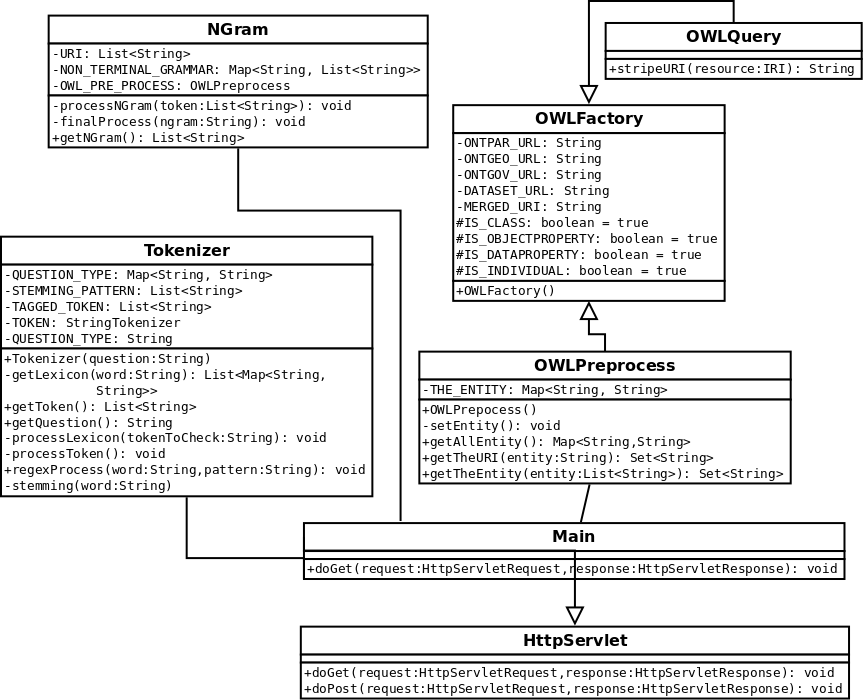
\includegraphics[width=1\textwidth]{class_diagram}
    \caption{Diagram kelas aplikasi}
    \label{fig:class_diagram}
\end{figure}

\subsection{Diagram \emph{activity}}
\subsection{Diagram \emph{sequence}}